% Created 2024-02-22 Thu 21:42
% Intended LaTeX compiler: pdflatex
\documentclass[t]{beamer}
\usepackage[utf8]{inputenc}
\usepackage[T1]{fontenc}
\usepackage{graphicx}
\usepackage{longtable}
\usepackage{wrapfig}
\usepackage{rotating}
\usepackage[normalem]{ulem}
\usepackage{amsmath}
\usepackage{amssymb}
\usepackage{capt-of}
\usepackage{hyperref}
\usepackage{fontspec}
\usepackage{polyglossia}
\setmainlanguage[babelshorthands=true]{german}
\usepackage{hyperref}
\usepackage{color}
\usepackage{xcolor}
\usepackage[misc]{ifsym}
\definecolor{darkblue}{rgb}{0,0,.5}
\definecolor{darkgreen}{rgb}{0,.5,0}
\definecolor{islamicgreen}{rgb}{0.0, 0.56, 0.0}
\definecolor{darkred}{rgb}{0.5,0,0}
\definecolor{mintedbg}{rgb}{0.95,0.95,0.95}
\definecolor{arsenic}{rgb}{0.23, 0.27, 0.29}
\definecolor{prussianblue}{rgb}{0.0, 0.19, 0.33}
\definecolor{coolblack}{rgb}{0.0, 0.18, 0.39}
\hypersetup{colorlinks=true, breaklinks=true, anchorcolor=blue,linkcolor=white, citecolor=islamicgreen, filecolor=darkred,  urlcolor=darkblue}
\usepackage{booktabs}
\usepackage{pgf}
\usepackage{minted}
\RequirePackage{fancyvrb}
\DefineVerbatimEnvironment{verbatim}{Verbatim}{fontsize=\scriptsize}
\usetheme{Amsterdam}
\author{Göran Kirchner\thanks{e\_kirchnerg@doz.hwr-berlin.de}}
\date{2024-02-23}
\title{Funktionale Programmierung in F\# (1)}
\subtitle{Erste Schritte in F\#}
\hypersetup{
 pdfauthor={Göran Kirchner},
 pdftitle={Funktionale Programmierung in F\# (1)},
 pdfkeywords={},
 pdfsubject={},
 pdfcreator={Emacs 29.1 (Org mode 9.6.6)}, 
 pdflang={English}}
\begin{document}

\maketitle

\section{Organisatorisches }
\label{sec:org5fcc24f}

\begin{frame}[label={sec:org00f1a1b}]{Organisatorisches}
\begin{itemize}
\item Termine
\begin{itemize}
\item\relax [23.02, 15.03, 05.04, 19.04, 03.05]
\end{itemize}
\item Bewertung
\begin{itemize}
\item .50: Hausaufgaben (10)
\item .25: Programmieraufgabe (in der vorvorletzten Einheit)
\item .25: Test (multiple choice, in der letzten Einheit)
\end{itemize}
\item Folien und Code auf \href{https://github.com/kirchnergo/course.2023.hwr.fun}{github.com/kirchnergo/course.2024.hwr.fun}
\end{itemize}
\end{frame}

\begin{frame}[label={sec:orgb0c2084}]{Was ist F\#}
F\# ist eine funktionale Programmiersprache, die das Schreiben von korrektem und verwaltbarem Code erleichtert.
In F\# können Typen und Funktionen geschrieben werden, deren Typen automatisch generalisiert werden. Dies ermöglicht es, sich auf die Problemdomäne zu konzentrieren und die Daten zu bearbeiten, statt sich um die Details der Programmierung zu kümmern.

F\# verfügt über zahlreiche Features, einschließlich:
\begin{itemize}
\item Leichtgewichtige Syntax
\item Standardmäßig unveränderliche Werte
\item Typrückschluss und automatische Generalisierung
\item Funktionen erster Klasse
\item Musterabgleich
\item Asynchrone Programmierung
\end{itemize}
\end{frame}

\begin{frame}[label={sec:org85d5547},fragile]{So sieht F\# aus}
 \begin{minted}[bgcolor=mintedbg,frame=none,framesep=0pt,mathescape=true,fontsize=\scriptsize,breaklines=true,linenos=false,numbersep=5pt,gobble=0]{fsharp}
open System // Gets access to functionality in System namespace.

// Defines a function that takes a name and produces a greeting.
let getGreeting name =
    sprintf "Hello, %s! Isn't F# great?" name

let main args =
    // Defines a list of names
    let names = [ "Don"; "Julia"; "Xi" ]
    // Prints a greeting for each name!
    names
    |> List.map getGreeting
    |> List.iter (fun greeting -> printfn "%s" greeting)
    0
\end{minted}
\end{frame}

\begin{frame}[label={sec:orgb9d1ab7}]{Programm}
\begin{enumerate}
\item Einführung \& Erste Schritte
\item Grundlagen \& ROP (Railway Oriented Programming)
\item Grundlagen \& DDD (Domain Driven Design)
\item Property-Based Testing
\item Parser Combinators
\end{enumerate}
\end{frame}

\begin{frame}[label={sec:org05f94ee}]{Einführung \& Erste Schritte (1)}
\begin{itemize}
\item Werkzeuge (VS Code, git, dotnet)
\item Datentypen
\item Collections
\item Pattern Matching
\item Funktionen
\end{itemize}
\end{frame}

\begin{frame}[label={sec:org09450d3}]{Grundlagen \& ROP - Railway Oriented Programming (2)}
\begin{itemize}
\item Fehlende Daten (option)
\item Umgang mit Fehlern
\item Railway Oriented Programming
\item (Asynchron \& Parallel)
\end{itemize}
\end{frame}

\begin{frame}[label={sec:org2f95d98}]{Grundlagen \& DDD (Domain Driven Design) (3)}
\begin{itemize}
\item Immutability
\item Algebraische Datentypen, Record Types (Wiederholung)
\item Typen-getriebene Programmierung (Type Driven Design)
\item (Klassen)
\item\relax [Programmieraufgabe!]
\end{itemize}
\end{frame}

\begin{frame}[label={sec:org8070232}]{Property-Based Testing (4)}
\begin{itemize}
\item Testing
\item Property-Based Testing
\item Diamond-Kata?
\item (Performance)
\end{itemize}
\end{frame}

\begin{frame}[label={sec:org62709a1}]{Parser Combinators (5)}
\begin{itemize}
\item Parser Combinators verstehen
\item FParsec
\item\relax [Test!]
\end{itemize}
\end{frame}


\section{Werkzeuge }
\label{sec:orgd4c8531}

\begin{frame}[label={sec:orgef5398e}]{Benötigte Software}
\begin{itemize}
\item \href{https://dotnet.microsoft.com/download}{.Net Core SDK 8.0}
\item \href{https://git-scm.com/}{git}
\item \href{https://code.visualstudio.com/}{Visual Studio Code}
\begin{itemize}
\item \href{http://ionide.io/}{ionide.io}
\end{itemize}
\item \href{https://try.fsharp.org/}{try.fsharp.org} oder \href{https://fable.io/repl/}{fable.io/repl/}
\item \href{https://exercism.io/}{exercism.io}
\item (\href{https://github.com/}{github.com})
\end{itemize}
\end{frame}

\begin{frame}[label={sec:orga1b5fe3}]{Übung 1}
\begin{itemize}
\item Installation überprüfen
\begin{itemize}
\item dotnet core
\item git
\item code (VS Code)
\item exercism
\end{itemize}
\end{itemize}
\end{frame}

\begin{frame}[label={sec:org6ff8284},fragile]{Lösungen 1}
 \scriptsize
\begin{minted}[bgcolor=mintedbg,frame=none,framesep=0pt,mathescape=true,fontsize=\scriptsize,breaklines=true,linenos=false,numbersep=5pt,gobble=0]{shell}
. /usr/local/opt/asdf/asdf.sh
dotnet --version
\end{minted}

\begin{verbatim}
8.0.101
\end{verbatim}


\begin{minted}[bgcolor=mintedbg,frame=none,framesep=0pt,mathescape=true,fontsize=\scriptsize,breaklines=true,linenos=false,numbersep=5pt,gobble=0]{shell}
git --version
\end{minted}

\begin{verbatim}
git version 2.39.3 (Apple Git-145)
\end{verbatim}



\begin{minted}[bgcolor=mintedbg,frame=none,framesep=0pt,mathescape=true,fontsize=\scriptsize,breaklines=true,linenos=false,numbersep=5pt,gobble=0]{shell}
code --version
\end{minted}

\begin{tabular}{l}
1.85.2\\[0pt]
8b3775030ed1a69b13e4f4c628c612102e30a681\\[0pt]
x64\\[0pt]
\end{tabular}

\begin{minted}[bgcolor=mintedbg,frame=none,framesep=0pt,mathescape=true,fontsize=\scriptsize,breaklines=true,linenos=false,numbersep=5pt,gobble=0]{shell}
exercism version
\end{minted}

\begin{verbatim}
exercism version 3.3.0
\end{verbatim}
\end{frame}

\begin{frame}[label={sec:orgcce3af6}]{Übung 2}
\begin{itemize}
\item \href{https://docs.microsoft.com/de-de/dotnet/fsharp/get-started/get-started-command-line}{Erste Schritte in F\# mit der .NET Core-CLI}
\item Erstelle ein F\# Projekt
\begin{itemize}
\item Untersuche das Ergebnis
\item Starte das Programm
\end{itemize}
\end{itemize}
\end{frame}

\begin{frame}[label={sec:org1385edc},fragile]{Lösung 2}
 \begin{minted}[bgcolor=mintedbg,frame=none,framesep=0pt,mathescape=true,fontsize=\scriptsize,breaklines=true,linenos=false,numbersep=5pt,gobble=0]{shell}
dotnet new sln -o FSNetCore
cd FSNetCore

dotnet new classlib -lang "F#" -o src/Library
dotnet add src/Library/Library.fsproj package Newtonsoft.Json
dotnet sln add src/Library/Library.fsproj

dotnet new console -lang "F#" -o src/App
dotnet add src/App/App.fsproj reference \
    src/Library/Library.fsproj
dotnet sln add src/App/App.fsproj

cd src/App
dotnet run Hello World
\end{minted}
\end{frame}

\begin{frame}[label={sec:org2472499},fragile]{git}
 \begin{itemize}
\item \href{https://git-scm.com/}{git}
\begin{minted}[bgcolor=mintedbg,frame=none,framesep=0pt,mathescape=true,fontsize=\scriptsize,breaklines=true,linenos=false,numbersep=5pt,gobble=0]{shell}
git init
git clone '<repo>'
git status
git add .
git commit -m 'good message'
git log
\end{minted}
\item \href{https://github.com/}{github.com}
\begin{itemize}
\item \href{https://help.github.com/en/github/getting-started-with-github/create-a-repo}{getting-started-with-github/create-a-repo}
\end{itemize}
\item \href{https://gitignore.io/}{gitignore.io}
\item \href{https://chris.beams.io/posts/git-commit/}{How to Write a Git Commit Message}
\end{itemize}
\end{frame}

\begin{frame}[label={sec:orgfdc0ad6},fragile]{Übung 3}
 \begin{itemize}
\item Initialisiere ein git-Repo (z.B. \texttt{course.2024.hwr.fun})
\begin{itemize}
\item (pull von github)
\item Committe eine Änderung
\item Betrachte die Historie
\item (push nach github)
\end{itemize}
\item clone \href{https://github.com/kirchnergo/course.2024.hwr.fun}{github.com/kirchnergo/course.2024.hwr.fun}
\end{itemize}
\end{frame}

\begin{frame}[label={sec:orgb86bc36},fragile]{exercism}
 \begin{itemize}
\item \href{https://exercism.io/about}{exercism.io/about}
\item Konfiguration
\begin{minted}[bgcolor=mintedbg,frame=none,framesep=0pt,mathescape=true,fontsize=\scriptsize,breaklines=true,linenos=false,numbersep=5pt,gobble=0]{shell}
exercism configure --token=99ada440-..-0be7ce2cfe40
exercusm configure --workspace=/foo
\end{minted}
\item Download und Sumbit
\begin{minted}[bgcolor=mintedbg,frame=none,framesep=0pt,mathescape=true,fontsize=\scriptsize,breaklines=true,linenos=false,numbersep=5pt,gobble=0]{shell}
exercism download --exercise=hello-world --track=fsharp
exercism submit /path/to/file [/path/to/file2 ...]
\end{minted}
\end{itemize}
\end{frame}

\begin{frame}[label={sec:orgf36964b}]{Übung 4}
\begin{itemize}
\item Konfiguriere exercism.io
\item Lade die Hello-World-Aufgabe von exercism.io runter
\begin{itemize}
\item Lass alle Tests laufen
\item Löse die Aufgabe
\item Submitte das Ergebnis
\end{itemize}
\item commit \& push
\end{itemize}
\end{frame}

\begin{frame}[label={sec:org062bcc7},fragile]{Lösung 4}
 \scriptsize
\begin{minted}[bgcolor=mintedbg,frame=none,framesep=0pt,mathescape=true,fontsize=\scriptsize,breaklines=true,linenos=false,numbersep=5pt,gobble=0]{shell}
exercism download --exercise=hello-world --track=fsharp
\end{minted}

\begin{minted}[bgcolor=mintedbg,frame=none,framesep=0pt,mathescape=true,fontsize=\scriptsize,breaklines=true,linenos=false,numbersep=5pt,gobble=0]{fsharp}
module HelloWorld =
  let hello: string = "Hello, World!"
\end{minted}

\begin{verbatim}
module HelloWorld =
  val hello: string = "Hello, World!"
\end{verbatim}


\begin{minted}[bgcolor=mintedbg,frame=none,framesep=0pt,mathescape=true,fontsize=\scriptsize,breaklines=true,linenos=false,numbersep=5pt,gobble=0]{shell}
dotnet test
exercism submit HelloWorld.fs
\end{minted}
\end{frame}

\begin{frame}[label={sec:org8ca7488}]{Pause}
\begin{block}{}
A language that doesn’t affect the way you think about programming, is not worth knowing.

\null\hfill-- Alan Perlis
\end{block}
\end{frame}


\section{Datentypen }
\label{sec:org843259c}

\begin{frame}[label={sec:orge7e2bf4},fragile]{Elementare Datentypen}
 \scriptsize
\begin{minted}[bgcolor=mintedbg,frame=none,framesep=0pt,mathescape=true,fontsize=\scriptsize,breaklines=true,linenos=false,numbersep=5pt,gobble=0]{fsharp}
let s = "hello"  // string
let i = 42       // int
let f = 3.141    // float
let b = true     // bool
let l = [1;2;3]  // list
printfn "%s, %i, %f, %g, %b, %A" s i f f b l
\end{minted}

\begin{verbatim}
hello, 42, 3.141000, 3.141, true, [1; 2; 3]
val s: string = "hello"
val i: int = 42
val f: float = 3.141
val b: bool = true
val l: int list = [1; 2; 3]
val it: unit = ()
\end{verbatim}
\end{frame}

\begin{frame}[label={sec:org312fa74},fragile]{Tuple}
 \begin{minted}[bgcolor=mintedbg,frame=none,framesep=0pt,mathescape=true,fontsize=\scriptsize,breaklines=true,linenos=false,numbersep=5pt,gobble=0]{fsharp}
let t1 = (1, 2)
let t2 = ("one", "two", "three")
let t3 = (10, 10.0, "ten")
printfn "%A, %A %A" t1 t2 t3
\end{minted}

\begin{verbatim}
(1, 2), ("one", "two", "three") (10, 10.0, "ten")
val t1: int * int = (1, 2)
val t2: string * string * string = ("one", "two", "three")
val t3: int * float * string = (10, 10.0, "ten")
val it: unit = ()
\end{verbatim}
\end{frame}

\begin{frame}[label={sec:org978237b},fragile]{Discriminated Union}
 \begin{minted}[bgcolor=mintedbg,frame=none,framesep=0pt,mathescape=true,fontsize=\scriptsize,breaklines=true,linenos=false,numbersep=5pt,gobble=0]{fsharp}
type Suit = 
    | Hearts 
    | Clubs 
    | Diamonds 
    | Spades
type Rank = 
    | Value of int
    | Ace
    | King
    | Queen
    | Jack
    static member GetAllRanks() = 
        [ yield Ace
          for i in 2 .. 10 do yield Value i
          yield Jack; yield Queen; yield King ]
\end{minted}
\end{frame}

\begin{frame}[label={sec:org1090811},fragile]{Record Types}
 \begin{itemize}
\item Gleichheit bei gleichen Werten 
\begin{itemize}
\item bei Klassen: Gleichheit bei gleicher Referenz!
\end{itemize}
\item Können rekursiv sein
\end{itemize}

\begin{minted}[bgcolor=mintedbg,frame=none,framesep=0pt,mathescape=true,fontsize=\scriptsize,breaklines=true,linenos=false,numbersep=5pt,gobble=0]{fsharp}
type Card = { Suit: Suit; Rank: Rank }

/// This computes a list representing all the cards in the deck.
let fullDeck = 
    [ for suit in [Hearts; Diamonds; Clubs; Spades] do
              for rank in Rank.GetAllRanks() do 
                  yield {Suit=suit; Rank=rank} ];;
fullDeck |> Seq.length
\end{minted}

\begin{verbatim}
fullDeck |> Seq.length;;
val it: int = 52
\end{verbatim}
\end{frame}


\section{Collections }
\label{sec:org4f2c1d3}

\begin{frame}[label={sec:org84e12cf},fragile]{Lists, Array, Seq}
 \scriptsize

\begin{minted}[bgcolor=mintedbg,frame=none,framesep=0pt,mathescape=true,fontsize=\scriptsize,breaklines=true,linenos=false,numbersep=5pt,gobble=0]{fsharp}
let list1 = [ 1; 2; 3 ]
let list2 = [ for i in 1 .. 8 -> i*i ]
let list3 = []
let list4 = 100 :: list2
let list5 = list1 @ list2
let list6 = [1 .. 10]
let array1 = [| 1; 2; 3 |]
let seq1 = seq {1 .. 3}
printfn "%A, %A, %A" list1 array1 seq1
\end{minted}

\begin{verbatim}
[1; 2; 3], [|1; 2; 3|], seq [1; 2; 3]
val list1: int list = [1; 2; 3]
val list2: int list = [1; 4; 9; 16; 25; 36; 49; 64]
val list3: 'a list
val list4: int list = [100; 1; 4; 9; 16; 25; 36; 49; 64]
val list5: int list = [1; 2; 3; 1; 4; 9; 16; 25; 36; 49; 64]
val list6: int list = [1; 2; 3; 4; 5; 6; 7; 8; 9; 10]
val array1: int array = [|1; 2; 3|]
val seq1: int seq
val it: unit = ()
\end{verbatim}
\end{frame}

\begin{frame}[label={sec:org71a47af},fragile]{Unendliche Sequenzen :)}
 \begin{minted}[bgcolor=mintedbg,frame=none,framesep=0pt,mathescape=true,fontsize=\scriptsize,breaklines=true,linenos=false,numbersep=5pt,gobble=0]{fsharp}
/// A random-number generator 
let rand = System.Random() ;;
/// An infinite sequence of numbers
let randomNumbers = seq { while true do yield rand.Next(100000) };;
/// The first 10 random numbers, sorted
let firstTenRandomNumbers = 
    randomNumbers
    |> Seq.take 10 
    |> Seq.sort
    |> Seq.toList;;
firstTenRandomNumbers
\end{minted}

\begin{verbatim}
firstTenRandomNumbers;;
val it: int list =
  [29417; 36207; 43823; 57159; 68030; 83216; 85562; 90240; 90637; 98558]
\end{verbatim}
\end{frame}

\begin{frame}[label={sec:orgddd762a}]{Collection Functions}
\begin{center}
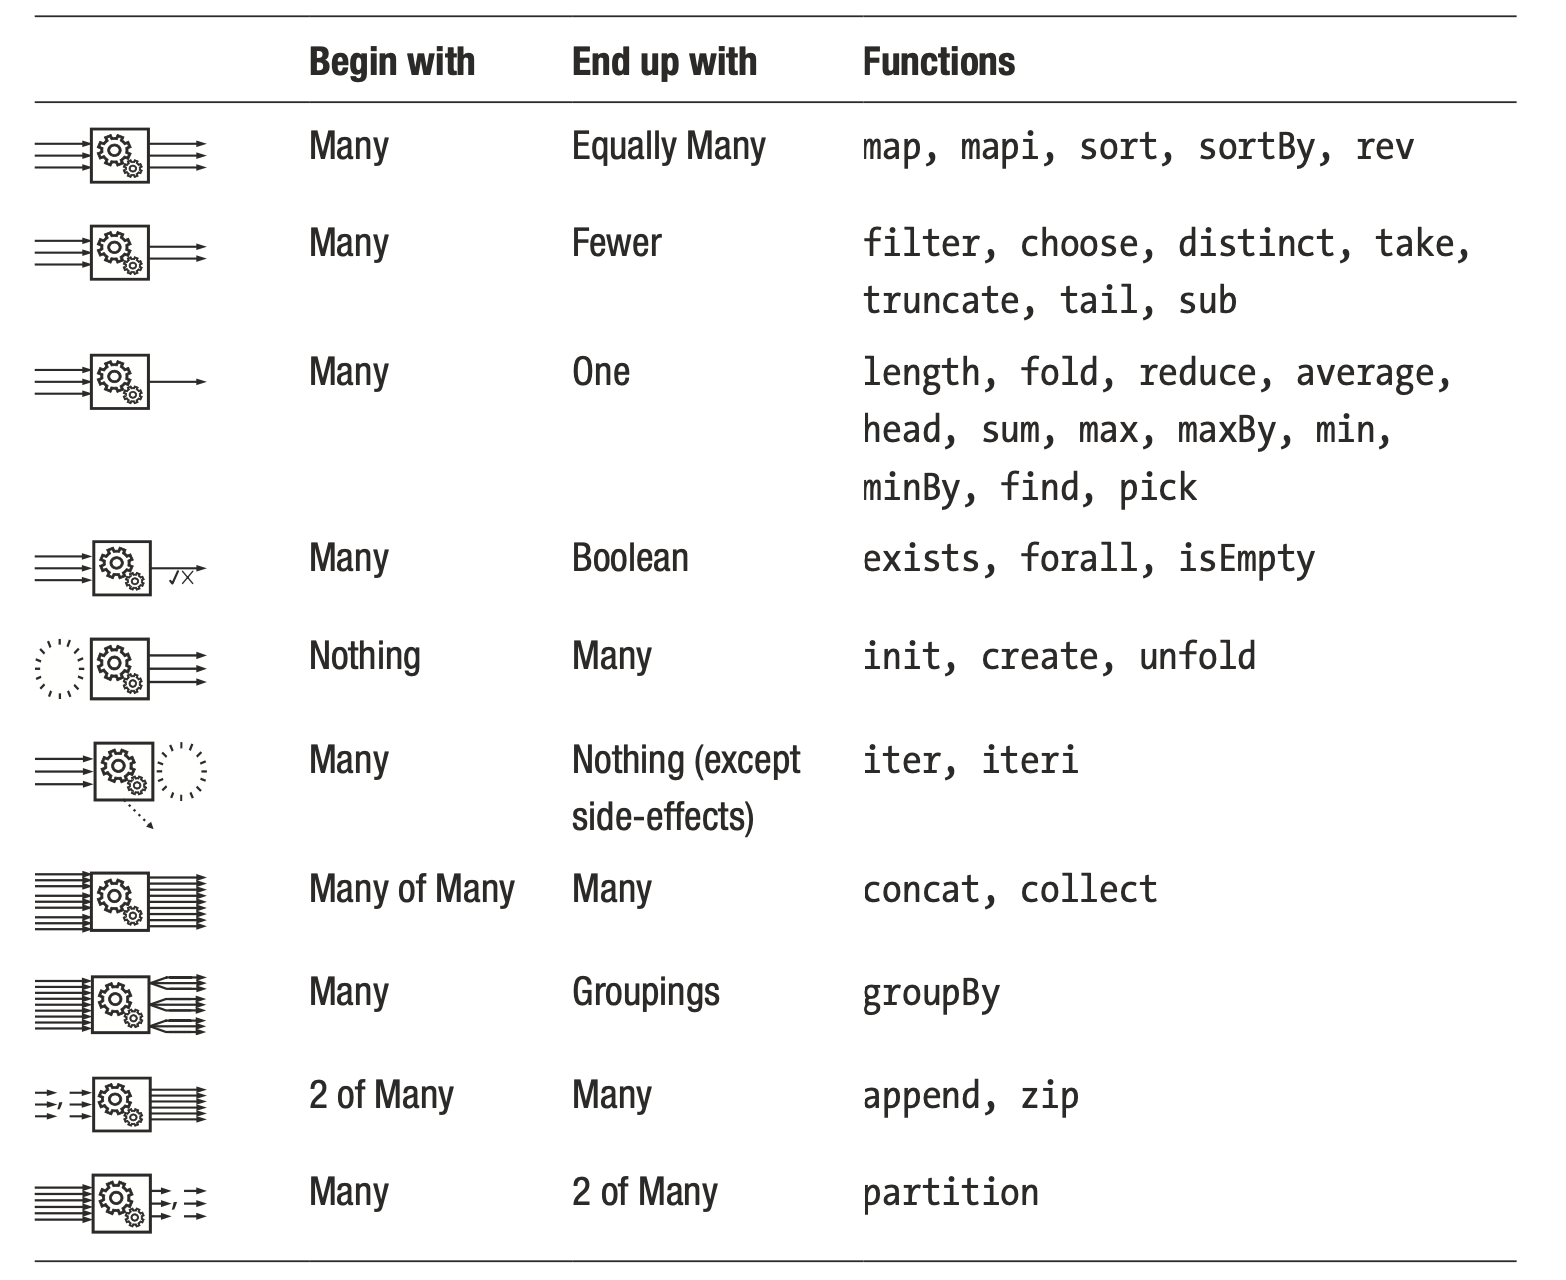
\includegraphics[height=200]{../img/CollectionFunctions.png}
\label{fig:collection-functions}
\end{center}
\end{frame}

\begin{frame}[label={sec:org69444ff},fragile]{Mapping (1)}
 \begin{minted}[bgcolor=mintedbg,frame=none,framesep=0pt,mathescape=true,fontsize=\scriptsize,breaklines=true,linenos=false,numbersep=5pt,gobble=0]{fsharp}
let primeCubes = List.map (fun n -> n * n * n) [2;3;5;7;11;13;17;19]
primeCubes
\end{minted}

\begin{verbatim}
val primeCubes: int list = [8; 27; 125; 343; 1331; 2197; 4913; 6859]
val it: int list = [8; 27; 125; 343; 1331; 2197; 4913; 6859]
\end{verbatim}


\begin{minted}[bgcolor=mintedbg,frame=none,framesep=0pt,mathescape=true,fontsize=\scriptsize,breaklines=true,linenos=false,numbersep=5pt,gobble=0]{fsharp}
/// Get the contents of the URL via a web request
let getAsync (url:string) = 
    async {
        let httpClient = new System.Net.Http.HttpClient()
        let! response = httpClient.GetAsync(url) |> Async.AwaitTask
        response.EnsureSuccessStatusCode () |> ignore
        return! response.Content.ReadAsStringAsync() |> Async.AwaitTask
    } |> Async.RunSynchronously
\end{minted}

\begin{verbatim}
val getAsync: url: string -> string
\end{verbatim}
\end{frame}

\begin{frame}[label={sec:org398a00f},fragile]{Mapping (2)}
 \tiny
\begin{minted}[bgcolor=mintedbg,frame=none,framesep=0pt,mathescape=true,fontsize=\scriptsize,breaklines=true,linenos=false,numbersep=5pt,gobble=0]{fsharp}
let sites = ["http://www.bing.com"; "http://www.google.com"]
let fetch url = (url, getAsync url)
let ps = List.map fetch sites
let ls = List.map (fun (_,p) -> String.length p) ps
printfn "%A" ls
\end{minted}

\begin{verbatim}
[40151; 51450]
val sites: string list = ["http://www.bing.com"; "http://www.google.com"]
val fetch: url: string -> string * string
val ps: (string * string) list =
  [("http://www.bing.com",
    "<!doctype html><html lang="de" dir="ltr"><head><meta name="th"+[40090 chars]);
   ("http://www.google.com",
    "<!doctype html><html itemscope="" itemtype="http://schema.org"+[51389 chars])]
val ls: int list = [40151; 51450]
val it: unit = ()
\end{verbatim}
\end{frame}


\begin{frame}[label={sec:orgafb33fb},fragile]{Folding}
 \begin{minted}[bgcolor=mintedbg,frame=none,framesep=0pt,mathescape=true,fontsize=\scriptsize,breaklines=true,linenos=false,numbersep=5pt,gobble=0]{fsharp}
let fold1 = List.fold (fun acc x -> acc + x) 0 [1..10]
let fold2 = [1..100] |> List.fold (+) 0
let fold3 = (0, [1..1000]) ||> List.fold (+)
printfn "%i, %i, %i" fold1 fold2 fold3
\end{minted}

\begin{verbatim}
55, 5050, 500500
val fold1: int = 55
val fold2: int = 5050
val fold3: int = 500500
val it: unit = ()
\end{verbatim}
\end{frame}

\begin{frame}[label={sec:org1f91c07}]{Pause}
\begin{block}{}
Computers are useless. They can only give you answers.

\null\hfill-- Pablo Picasso
\end{block}
\end{frame}


\section{Pattern Matching }
\label{sec:orgeba6c48}

\begin{frame}[label={sec:org589ae59},fragile]{Basics}
 \begin{minted}[bgcolor=mintedbg,frame=none,framesep=0pt,mathescape=true,fontsize=\scriptsize,breaklines=true,linenos=false,numbersep=5pt,gobble=0]{fsharp}
let matchInt i =
    match i with
    | 1 -> printfn "One"
    | 2 -> printfn "Two"
    | _ -> printfn "Other"  // "_" is a wildcard

matchInt 1
matchInt 2
matchInt 77
\end{minted}

\begin{verbatim}
One
Two
Other
val matchInt: i: int -> unit
val it: unit = ()
\end{verbatim}
\end{frame}

\begin{frame}[label={sec:org10a8335},fragile]{When Guards}
 \begin{minted}[bgcolor=mintedbg,frame=none,framesep=0pt,mathescape=true,fontsize=\scriptsize,breaklines=true,linenos=false,numbersep=5pt,gobble=0]{fsharp}
let caseSwitch input =
    match input with
    | 1 -> printfn "One"
    | 2 -> printfn "A couple"
    | x when x < 12 -> printfn "Less than a dozen" 
    | x when x = 12 -> printfn "A dozen"
    | _ -> printfn "More than a dozen"

caseSwitch 2
caseSwitch 5
caseSwitch 12
caseSwitch 18
\end{minted}

\begin{verbatim}
A couple
Less than a dozen
A dozen
More than a dozen
val caseSwitch: input: int -> unit
val it: unit = ()
\end{verbatim}
\end{frame}

\begin{frame}[label={sec:org20c4c2a},fragile]{Matching Tuples (1)}
 \begin{minted}[bgcolor=mintedbg,frame=none,framesep=0pt,mathescape=true,fontsize=\scriptsize,breaklines=true,linenos=false,numbersep=5pt,gobble=0]{fsharp}
let extremes (s : seq<_>) = 
    s |> Seq.min,
    s |> Seq.max

let l, h = [1; 2; 9; 3; -1] |> extremes
(l,h)
\end{minted}

\begin{verbatim}
val extremes: s: 'a seq -> 'a * 'a when 'a: comparison
val l: int = -1
val h: int = 9
val it: int * int = (-1, 9)
\end{verbatim}
\end{frame}

\begin{frame}[label={sec:orgd1eee75},fragile]{Matching Tuples (2)}
 \begin{minted}[bgcolor=mintedbg,frame=none,framesep=0pt,mathescape=true,fontsize=\scriptsize,breaklines=true,linenos=false,numbersep=5pt,gobble=0]{fsharp}
open System
let tryParseInt (s:string) =
    match System.Int32.TryParse(s) with 
    | true, i -> Some i
    | false, _ -> None

let a = "30" |> tryParseInt // Some 30
let b = "3X" |> tryParseInt // None
(a,b)
\end{minted}

\begin{verbatim}
val tryParseInt: s: string -> int option
val a: int option = Some 30
val b: int option = None
val it: int option * int option = (Some 30, None)
\end{verbatim}
\end{frame}

\begin{frame}[label={sec:orga94dda4},fragile]{Matching Records}
 \begin{minted}[bgcolor=mintedbg,frame=none,framesep=0pt,mathescape=true,fontsize=\scriptsize,breaklines=true,linenos=false,numbersep=5pt,gobble=0]{fsharp}
type Track = { Title : string; Artist : string } ;;
let songs = [ { Title = "Summertime"; Artist = "Ray Barretto" };
      { Title = "La clave, maraca y guiro";
        Artist = "Chico Alvarez" };
      { Title = "Summertime";
        Artist = "DJ Jazzy Jeff & The Fresh Prince" } ] ;;
let dist = 
    songs 
    |> Seq.map (fun s -> match s with | {Title = title} -> title) 
    |> Seq.distinct |> Seq.toList
dist
\end{minted}

\begin{verbatim}
let dist = 
    songs 
    |> Seq.map (fun s -> match s with | {Title = title} -> title) 
    |> Seq.distinct |> Seq.toList
dist;;
val dist: string list = ["Summertime"; "La clave, maraca y guiro"]
val it: string list = ["Summertime"; "La clave, maraca y guiro"]
\end{verbatim}
\end{frame}

\begin{frame}[label={sec:org30caa54},fragile]{Matching Lists}
 \begin{minted}[bgcolor=mintedbg,frame=none,framesep=0pt,mathescape=true,fontsize=\scriptsize,breaklines=true,linenos=false,numbersep=5pt,gobble=0]{fsharp}
let caseList l = 
    match l with
    | [] -> printfn "An empty pond" 
    | [fish] -> printfn "A pond with one fish only: %s" fish 
    | head::tail -> printfn "A pond with one fish: \
         %s (and %i more fish)" head (tail |> List.length)

caseList []
caseList ["One fish"]
caseList ["One fish"; "Two fish"; "Red fish" ]
caseList ["One fish"; "Two fish"; "Red fish"; "Blue fish" ]
\end{minted}

\begin{verbatim}
An empty pond
A pond with one fish only: One fish
A pond with one fish: One fish (and 2 more fish)
A pond with one fish: One fish (and 3 more fish)
val caseList: l: string list -> unit
val it: unit = ()
\end{verbatim}
\end{frame}

\begin{frame}[label={sec:orgecef492},fragile]{Active Patterns (|?|)}
 \scriptsize
\begin{minted}[bgcolor=mintedbg,frame=none,framesep=0pt,mathescape=true,fontsize=\scriptsize,breaklines=true,linenos=false,numbersep=5pt,gobble=0]{fsharp}
let (|Even|Odd|) input = if input % 2 = 0 then Even else Odd
\end{minted}

\begin{verbatim}
val (|Even|Odd|) : input: int -> Choice<unit,unit>
\end{verbatim}


\begin{minted}[bgcolor=mintedbg,frame=none,framesep=0pt,mathescape=true,fontsize=\scriptsize,breaklines=true,linenos=false,numbersep=5pt,gobble=0]{fsharp}
let TestNumber input =
   match input with
   | Even -> printfn "%d is even" input
   | Odd -> printfn "%d is odd" input

TestNumber 7
TestNumber 8
TestNumber 9
\end{minted}

\begin{verbatim}
7 is odd
8 is even
9 is odd
val TestNumber: input: int -> unit
val it: unit = ()
\end{verbatim}
\end{frame}

\begin{frame}[label={sec:org298f164}]{Pause}
\begin{block}{}
Any fool can write code that a computer can understand. 
Good programmers write code that humans can understand.

\null\hfill-- Martin Fowler
\end{block}
\end{frame}


\section{Funktionen }
\label{sec:org93bd31e}

\begin{frame}[label={sec:orgf0461b1},fragile]{Basics}
 \begin{minted}[bgcolor=mintedbg,frame=none,framesep=0pt,mathescape=true,fontsize=\scriptsize,breaklines=true,linenos=false,numbersep=5pt,gobble=0]{fsharp}
let squareIt1 n = n * n
let squareIt2 = fun n -> n * n
let r1 = squareIt1 8
let r2 = squareIt2 9

let listOfFunctions = [squareIt1; squareIt2]
for fn in listOfFunctions do
    let result = fn 100
    printfn "If 100 is the input, the output is %i" result
\end{minted}

\begin{verbatim}
If 100 is the input, the output is 10000
If 100 is the input, the output is 10000
val squareIt1: n: int -> int
val squareIt2: n: int -> int
val r1: int = 64
val r2: int = 81
val listOfFunctions: (int -> int) list =
  [<fun:listOfFunctions@1195-10>; <fun:listOfFunctions@1195-11>]
val it: unit = ()
\end{verbatim}
\end{frame}

\begin{frame}[label={sec:org0dc1ff9},fragile]{Rekursion}
 \begin{minted}[bgcolor=mintedbg,frame=none,framesep=0pt,mathescape=true,fontsize=\scriptsize,breaklines=true,linenos=false,numbersep=5pt,gobble=0]{fsharp}
/// Computes the greatest common factor of two integers.
///
/// Since all of the recursive calls are tail calls,
/// the compiler will turn the function into a loop,
/// which improves performance and reduces memory consumption.
let rec gcf a b =
    match a with
    | 0 -> b
    | a when a < b -> gcf a (b - a)
    | _ -> gcf (a - b) b

printfn "The Greatest Common Factor of 300 \
         and 620 is %d" (gcf 300 620)
\end{minted}

\begin{verbatim}
The Greatest Common Factor of 300 and 620 is 20
val gcf: a: int -> b: int -> int
val it: unit = ()
\end{verbatim}
\end{frame}

\begin{frame}[label={sec:org5bd3f27},fragile]{Partielle Anwendung}
 \scriptsize

\begin{minted}[bgcolor=mintedbg,frame=none,framesep=0pt,mathescape=true,fontsize=\scriptsize,breaklines=true,linenos=false,numbersep=5pt,gobble=0]{fsharp}
let add1 = (+) 1        
let r1 = add1 2   // result => 3
let multiplyBy2 = (*) 2
let r2 = multiplyBy2 3   // result => 6
let equals3 = (=) 3
let r3 = equals3 3   // result => true

printfn "%i, %i, %b" r1 r2 r3
\end{minted}

\begin{verbatim}
3, 6, true
val add1: (int -> int)
val r1: int = 3
val multiplyBy2: (int -> int)
val r2: int = 6
val equals3: (int -> bool)
val r3: bool = true
val it: unit = ()
\end{verbatim}
\end{frame}

\begin{frame}[label={sec:org3e8b512},fragile]{Composition}
 \scriptsize

\begin{minted}[bgcolor=mintedbg,frame=none,framesep=0pt,mathescape=true,fontsize=\scriptsize,breaklines=true,linenos=false,numbersep=5pt,gobble=0]{fsharp}
let negate x = -1 * x
let square x = x*x
let print x = printfn "The number is: %d" x

let snp x = print (negate (square x))
let ``sqr, neg, and print`` x = x |> square |> negate |> print
let snp' = square >> negate >> print

snp 9, ``sqr, neg, and print`` 10, snp' 11
\end{minted}

\begin{verbatim}
The number is: -81
The number is: -100
The number is: -121
val negate: x: int -> int
val square: x: int -> int
val print: x: int -> unit
val snp: x: int -> unit
val ``sqr, neg, and print`` : x: int -> unit
val snp': (int -> unit)
val it: unit * unit * unit = ((), (), ())
\end{verbatim}
\end{frame}


\section{Ende }
\label{sec:org1e98753}

\begin{frame}[label={sec:orgfe84010}]{Zusammenfassung}
\begin{itemize}
\item Wichtige Werkzeuge (git, dotnet, code)
\item Elementare Syntax
\item Funktionen, Pattern Matching, Discriminated Unions (DU)
\item Tuple, Record, List, Array, Seq
\item Was ist Funktionale Programmierung?
\end{itemize}
\end{frame}

\begin{frame}[label={sec:org75bbfd5}]{Links}
\begin{itemize}
\item \href{https://fsharp.org/}{fsharp.org}
\item \href{https://docs.microsoft.com/de-de/dotnet/fsharp/}{docs.microsoft.com/../dotnet/fsharp}
\item \href{https://en.wikipedia.org/wiki/F\_Sharp\_(programming\_language)}{wikipedia.org/../F Sharp (programming language)}
\item \href{https://en.wikipedia.org/wiki/List\_of\_programming\_languages\_by\_type\#Functional\_languages}{wikipedia.org/../List of programming languages by type\#Functional languages}
\item \href{https://sergeytihon.com/}{F\# weekly}
\item \href{https://fsharpforfunandprofit.com/}{fsharpforfunandprofit.com}
\item \href{https://www.tutorialspoint.com/fsharp/index.htm}{tutorialspoint.com/fsharp}
\item \href{http://www.rosettacode.org/}{rosettacode.org}
\end{itemize}
\end{frame}

\begin{frame}[label={sec:org9222f66}]{Hausaufgabe}
\begin{itemize}
\item[{$\square$}] \href{https://git-scm.com/docs/gittutorial}{git Tutorial}
\item[{$\square$}] \href{https://docs.microsoft.com/de-de/dotnet/fsharp/tour}{Tour durch F\#}
\item exercism.io (E-Mail bis 11.03, mit \emph{account}!)
\begin{itemize}
\item[{$\square$}] Two-Fer
\item[{$\square$}] Leap
\item[{$\square$}] Isogram
\item[{$\square$}] Sum Of Multiples
\end{itemize}
\end{itemize}
\end{frame}
\end{document}